\chapter{L'algorithme \texorpdfstring{$\rho$}{Rho} de Pollard «\texorpdfstring{\,}{\ }classique\texorpdfstring{\,}{\ }»}
    	\section{Présentation}
      Soit $G$ un groupe fini, cyclique, généré par $g$ et d'ordre $q$. Le problème du logarithme discret consiste, pour un élément $h$ appartenant à $G$, à trouver le logarithme discret de $g$ en base $h$, noté $\log_g(h)$, c'est-à-dire le plus petit entier positif $x$ tel que $g^x = h$.

    	L'algorithme $\rho$ de Pollard est une méthode capable de répondre à un tel problème. Durant toute la suite du rapport, on travaillera dans le sous-groupe de $(\mathbb{Z}/p\mathbb{Z})^*$ d'ordre $q$, avec $p$ et $q$ deux nombres premiers. L'algorithme consiste à construire une suite $(x_i)_{i \ge 0}$ d'éléments de $G$ tels que $x_{i+1} = f(x_i)$ avec $f$ une fonction allant de $G$ dans $G$. Cette fonction est choisie de telle sorte à rendre possible le traçage des exposants par rapport à $g$ et $h$. Cela signifie que les appels à la fonction $f$ permettent de définir très simplement deux suites d'entiers $(a_i)_{i \ge 0}$ et $(b_i)_{i \ge 0}$ tels que $x_i = g^{a_i} \cdot h^{b_i}$. On calcule les $x_i$ jusqu'à détecter une collision, c'est-à-dire deux indices $i$ et $j$ tels que $i \ne j$ et $x_i = x_j$. Il est alors facile de trouver $x$. En effet, on a~:

    	\begin{align*}
        x_i = x_j &\implies g^{a_i} \cdot h^{b_i} = g^{a_j} \cdot h^{b_j} \\
                  &\implies h^{b_i - b_j} = g^{a_j - a_i} \\
                  &\implies (b_i - b_j) \cdot \log_g(h) \equiv a_j - a_i \text{\ mod } q
      \end{align*}

      Si $b_i$ non congru à $b_j$ modulo $q$, alors $b_i - b_j$ est inversible dans $G$ et il suffit de calculer son inverse dans ce groupe pour trouver $\log_g(h)$.

    	Toutes les variantes de l'algorithme reposent sur ce principe, mais chacune possède sa propre fonction d'itération et sa méthode pour détecter une collision. Intéressons-nous tout d'abord à la méthode classique, telle que décrite dans le \textit{Handbook of Applied Cryptography} \autocite[106]{handbook}.

        \section{La fonction d'itération}
        Dans le cas général, on définit la fonction d'itération comme la fonction permettant de calculer les différents éléments de notre suite $(x_i)_{i \ge 0}$ de la façon suivante~: $x_0 = 1$ et pour $i \geq 0$,

        \begin{align*}
          x_{i+1} =
          \begin{cases}
            h \cdot x_i & \text{si } x_i \in S_1 \\
            x_i^2 & \text{si } x_i \in S_2 \\
            g \cdot x_i & \text{si } x_i \in S_3
          \end{cases}
        \end{align*}
        Ici, $S_1$, $S_2$ et $S_3$ sont obtenus en partitionnant le groupe $G$ en trois sous-ensembles selon une propriété facilement testable. Remarquons qu'on doit nécessairement avoir $1 \notin S_2$. En effet, comme $x_0 = 1$, choisir $1 \in S_2$ nous donnerait $x_i = 1$ pour tout $i$.

        On définit les suites ${(a_i)}_{i \geq 0}$ et ${(b_i)}_{i \geq 0}$ comme suit~: $a_0 = 0$, $b_0 = 0$, et pour $i \geq 0$,

        \begin{align*}
          a_{i+1} =
          \begin{cases}
            a_i                   & \text{si } x_i \in S_1 \\
            2a_i \text{\ mod q}    & \text{si } x_i \in S_2 \\
            a_i + 1 \text{\ mod q} & \text{si } x_i \in S_3
          \end{cases}
        \end{align*}

        \begin{align*}
          b_{i+1} =
          \begin{cases}
            b_i + 1 \text{\ mod q} & \text{si } x_i \in S_1 \\
            2b_i \text{\ mod q}    & \text{si } x_i \in S_2 \\
            b_i                   & \text{si } x_i \in S_3
          \end{cases}
        \end{align*}

        On obtient l'égalité suivante, valable pour tout $i \in \mathbb{N}$~:
        \begin{equation} \label{eq:1}
          x_i = g^{a_i} \cdot h^{b_i}
        \end{equation}

		Dans quelques rares cas, cette fonction d'itération ne permet pas de détecter une collision. Il suffit alors d'exécuter de nouveau l'algorithme en choisissant les entiers $a_0$ et $b_0$ aléatoirement dans l'intervalle $\mathopen{[}1,q-1\mathclose{]}$ et en posant $x_0 = g^{a_0} \cdot h^{b_0}$.

		A présent, montrons par récurrence que \eqref{eq:1} reste satisfaite pour toute valeur de $i \in \mathbb{N}$.

        \subsection*{Initialisation}

        Dans le cas général, pour $i = 0$, on a par définition $x_0 = 1$ et $a_0 = b_0 = 0$.

        \begin{align*}
          g^{a_0} \cdot h^{b_0} &= g^{0} \cdot h^{0} \\
                                &= 1 \cdot 1 \\
                                &= x_0
        \end{align*}

        Dans les quelques cas où $a_0$ et $b_0$ sont choisis aléatoirement dans $\mathopen{[}1,q-1\mathclose{]}$, $x_0 = g^{a_0} \cdot h^{b_0}$ par définition.

        La relation est donc toujours vérifiée au rang $0$.

        \subsection*{Hérédité}

        On suppose que la relation est vérifiée pour un certain rang $k \in \mathbb{N}$~: $x_k = g^{a_k} \cdot h^{b_k}$. Montrons que cela reste vrai au rang $k + 1$, c'est-à-dire que l'on a~:

        \begin{align*}
          x_{k+1} = g^{a_{k+1}} \cdot h^{b_{k+1}}
        \end{align*}

        On distingue trois cas possibles~:

        \underline{$x_{k} \in S_1$}
        \begin{align*}
          a_{k+1} &= a_k \\
          \text{\ et } b_{k+1} &= b_k + 1 \text{\ mod q}
        \end{align*}
        d'où
        \begin{align*}
          g^{a_{k+1}} \cdot h^{b_{k+1}} &= g^{a_k} \cdot h^{b_k} \cdot h \\
                                        &= x_k \cdot h & \text{(par l'hypothèse de récurrence)} \\
                                        &= x_{k+1} & \text{(car $x_k \in S_1$)}
        \end{align*}


        \underline{$x_{k} \in S_2$}
        \begin{align*}
          a_{k+1} &= 2a_k \text{\ mod q}\\
          \text{\ et } b_{k+1} &= 2b_k \text{\ mod q}
        \end{align*}
        d'où
        \begin{align*}
          g^{a_{k+1}} \cdot h^{b_{k+1}} &= g^{2a_k} \cdot h^{2b_k} \\
                                        &= {(g^{a_k} \cdot h^{a_k})}^2 \\
                                        &= {(x_k)}^2 & \text{(par l'hypothèse de récurrence)} \\
                                        &= x_{k+1} & \text{(car $x_k \in S_2$)}
        \end{align*}

        \underline{$x_{k} \in S_3$}
        \begin{align*}
          a_{k+1} &= a_k + 1 \text{\ mod q} \\
          \text{\ et } b_{k+1} &= b_k
        \end{align*}
        d'où
        \begin{align*}
          g^{a_{k+1}} \cdot h^{b_{k+1}} &= g \cdot g^{a_k} \cdot h^{b_k} \\
                                        &= g \cdot x_k & \text{(par l'hypothèse de récurrence)} \\
                                        &= x_{k+1} & \text{(car $x_k \in S_3$)}
        \end{align*}


        \subsection*{Conclusion}
        On a montré que pour $i = 0$, l'égalité~\ref{eq:1} est vérifiée.
        De plus, si elle est vraie au rang $k$, alors elle est vraie au rang $k+1$.

        Finalement, pour tout $i \in \mathbb{N}, x_i = g^{a_i} \cdot h^{b_i}$.

        \section{Collision et algorithme de Floyd}
        \label{chapter1:Floyd}
        Notre objectif est de détecter une collision, c'est-à-dire de trouver deux indices $i$ et $j$ avec $i \ne j$ tels que $x_i = x_j$. Une méthode naïve est de stocker tous les $x_i$ calculés et de les comparer les uns avec les autres, mais cette technique se révèle coûteuse, aussi bien en temps qu'en mémoire. Plusieurs algorithmes ont été développés afin de répondre à ces deux exigences. L'un d'eux est l'algorithme de détection de cycle de Floyd, aussi appelé algorithme du lièvre et de la tortue. Il est utilisé dans la version classique de l'algorithme \texorpdfstring{$\rho$}{Rho} de Pollard, et présente le double avantage d'être rapide et de demander peu de stockage en mémoire. Pour l'appliquer, il suffit de commencer par calculer la paire $(x_1, x_2)$ avant d'utiliser la fonction d'itération décrite précédemment pour calculer les paires $(x_i, x_{2i})$ à partir de la paire précédente. On s'arrête lorsqu'on trouve un indice $j$ tel que $x_j = x_{2j}$.

        Un tel entier existe nécessairement car le groupe $G$ sur lequel on travaille est fini. En effet, cela garantit que la suite des $x_i$ est ultimement périodique. On appelle pré-période et période de la suite les plus petits entiers $T$ et $C$ satisfaisant la propriété suivante.

        \[ x_{kC+T} = x_T \]

        On a alors~: $ x_{kC+i} = x_i, \forall i \ge T, \forall k \in \mathbb{N}$

        On peut donc représenter les valeurs de la suite $x_i$ par une droite et un cycle partageant un noeud en commun (situé à une extrêmité de la droite). La longueur de la droite correspond à la pré-période $T$ de la suite et le nombre d'éléments dans le cycle correspond à la période $C$. Les éléments de la droite sont numérotés de $-T$ à $0$, $0$ étant le noeud commun à la droite et au cycle. De la même manière, on numérote les noeuds du cycle par les entiers compris entre $0$ et $C-1$. On peut alors utiliser l'analogie suivante~: une tortue et un lièvre commencent en position $-T$ sur la droite. A chaque étape ils se déplacent respectivement de un et deux pas vers le noeud $0$. Une fois qu'ils ont atteint celui-ci, ils continuent de se déplacer à la même vitesse mais n'effectuent plus que des tours de cycle (dans le même sens et en allant du noeud $0$ au noeud $C-1$). Comme chaque noeud représente un nombre appartenant au groupe $G$, et qu'à une étape $i$ donnée la tortue est sur le noeud correspondant à la valeur $x_i$ et le lièvre sur le noeud correspondant à $x_{2i}$, il suffit que les deux animaux soient au même point au même moment pour qu'il y ait une collision. Nous allons à présent prouver que celle-ci survient alors que la tortue effectue son premier tour de cycle.

        \begin{figure}
          \center{}
          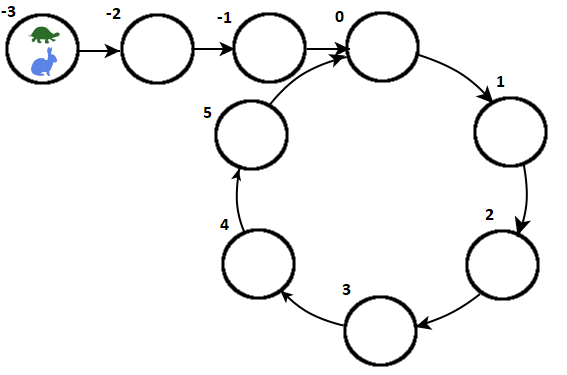
\includegraphics[scale=0.5]{Floyd.png}
          \caption{Algorithme de Floyd avec $T=3$ et $C=6$}
        \end{figure}

        La tortue commence en position $-T$, il lui faut précisément $T$ étapes pour qu'elle se trouve au début du cycle, soit en position $0$. A ce moment, le lièvre a avancé de $2 \cdot T$ pas, et il a déjà parcouru $T$ nœuds dans le cycle. Sa position dans celui-ci est donc donnée par le reste de la division euclidienne de $T$ par $C$.

        \begin{align*}
          \exists k \in \mathbb{N} \text{\ tel que } T = C \cdot k + r \text{\, avec } 0 \leq r < C, \text{d'où } T &\equiv r \text{\ mod } C
        \end{align*}

        Lorsque la tortue atteint pour la première fois le nœud $0$, le lièvre est alors en position $r$ dans le cycle. Si $r=0$, c'est terminé, car alors le lièvre et la tortue sont au même endroit. Supposons $r$ différent de $0$. On peut terminer en $C-r$ étapes supplémentaires.

        À l'issue de ces $C-r$ étapes, la tortue est en position $C-r$ dans le cycle. La position du lièvre est donnée par~:

        \begin{align*}
          r + 2 \cdot (C - r) &\equiv 2 \cdot C -r \text{\ mod } C \\
                              &\equiv C - r \text{\ mod } C
        \end{align*}

        Le lièvre et la tortue sont donc au même endroit et il y a collision, on peut trouver un indice $i$ tel que $x_i = x_{2i}$. De plus, on a pu terminer en $T + C - r$ étapes.

        A présent, nous allons voir comment implémenter la version classique de l'algorithme $\rho$ de Pollard.
